%% ============================================
%% ================ Preambule =================
%% ============================================
\documentclass[]{scrartcl}
\usepackage[margin = 0.5in]{geometry}

\usepackage[pdftex,unicode, 
colorlinks=true,
linkcolor = blue]{hyperref}	% нумерование страниц, ссылки!!!!ИМЕННО В ТАКОМ ПОРЯДКЕ СО СЛЕДУЮЩИМ ПАКЕТОМ
%\usepackage[warn]{mathtext}				% Поддержка русского текста в формулах
\usepackage[T1, T2A]{fontenc}			% Пакет выбора кодировки и шрифтов
\usepackage[utf8]{inputenc} 			% любая желаемая кодировка
\usepackage[english]{babel}		% поддержка русского языка
\usepackage{wrapfig}					% Плавающие картинки
\usepackage{amssymb, amsmath}			% стилевой пакет для формул
\usepackage{algorithm}
\usepackage{algorithmic} 


\ifpdf
\usepackage{cmap} 				% чтобы работал поиск по PDF
\usepackage[pdftex]{graphicx}
%\usepackage{pgfplotstable}		% Для вставки таблиц.
\pdfcompresslevel=9 			% сжимать PDF
\else
\usepackage{graphicx}
\fi

\graphicspath{{./figures/}}
\usepackage{subcaption}

%custom commands
\newcommand{\norm}[1]{\Vert{#1}\Vert}

%% ============================================
%% ================ Info =================
%% ============================================
\title{Neon: Nuclear Norm to Beat Muon}

\author{
  Alexey Kravatskiy\\
  \texttt{kravtskii.aiu@phystech.edu}
  \and
  Ivan Kozyrev\\
  \texttt{kozyrev.in@phystech.edu}
  \and
  Nikolay Kozlov \\
  \texttt{kozlov.na@phystech.edu}
  \and
  Alexander Vinogradov \\
  \texttt{vinogradov.am@phystech.edu}
}

%\author{\begin{tabular}{c c}
%	  	 Alexey Kravatsky & Nikolay Kozlov & Ivan Kozyrev \\
%		 \texttt{kravatskii.aiu@phystech.edu} & \texttt{kozlov.n?@phystech.edu} & \texttt{kozyrev.i?@phystech.edu}  
%		\end{tabular}}
\date{\today}

\begin{document}

\maketitle

\begin{abstract}
In this paper, we develop a new algorithm for optimization of functions of weight matrices, which are typical for training large language models. Changing spectral norm, which was used to derive Muon, to nuclear norm, we pose a new optimization problem for an update matrix, solution of which defines a novel algorithm we name Neon. To make it feasible, we use Lanczos algorithm to find a required step. After providing theoretical guarantees of Neon convergence, we compare performances of Neon, Muon, and Adam on training multilayer perceptron, convolutional neural network and NanoGPT.

\end{abstract}

\section{Idea}
The goal of the project is to make variations on Muon to speed it up. Recently, authors of \cite{bernstein2024oldoptimizernewnorm} have proposed to look at different optimizers as the solution of the optimization problem for an update. This approach can be utilized to derive Muon \cite{jordan2024muon}, a novel algorithm for fast training of neural networks. Instead of using spectral norm in the problem, we use nuclear norm to produce a new problem. %Then, we add momentum to update. After finalizing the algorithm, we test it on MLP, and, if results are satisfactory, on transformers (probably something from huggingface). The result will be a fast algorithm, which we will convert into a new optimizer class for PyTorch, as was done with Muon.%

\subsection{Problem (Project description)}

In this subsection, we provide a more detailed description of our idea and formulate it as a mathematical problem. The authors of \cite{bernstein2024oldoptimizernewnorm} suggest obtaining the update step as a solution to the optimization problem:
\begin{equation}
    \langle g, \delta w \rangle + \lambda \norm{\delta w}^2 \to \min_{\delta w}\,,
\end{equation}
where $w$ is the weight vector, $g$ is a gradient-like vector (e.g., obtained via momentum SGD), and $\norm{\cdot}$ represents a certain norm. Many popular optimizers, such as Adam (with exponential moving average disabled) and vanilla SGD, can be cast within this framework \cite{bernstein2024oldoptimizernewnorm}.

In large language models, most weights are structured as matrices, which offers additional opportunities for optimization. Let $W$ be the weight matrix of a linear layer, and $G$ be a gradient-like matrix. Then, the update step $\delta W$ can be obtained as a solution to the optimization problem:
\begin{equation}\label{eqn:opt_problem_mat}
  \langle G, \delta W \rangle + \lambda \norm{\delta W}^2 \to \min_{\delta W}\,,
\end{equation}
where $\norm{\cdot}$ denotes a certain matrix norm. By setting this norm to the RMS-to-RMS norm (a scaled version of the spectral norm), we recover the Muon optimizer \cite{bernstein2025deriving, bernstein2024oldoptimizernewnorm} with an update step defined by:
\begin{equation}\label{eqn:update_muon}
\delta W = - \frac{1}{\lambda}\sqrt{\frac{n}{m}}UV^T\,,
\end{equation}
where $m$ is the input dimension of the layer, $n$ is the output dimension, and $U$ and $V$ are obtained from the singular value decomposition of the gradient matrix $G = U \Sigma V$.

Motivated by the recent achievements of the Muon optimizer (e.g., \cite{liu2025muon}), we consider alternative choices of norms, specifically the kernel norm $\norm{\cdot}_*$ and a custom $F*$ norm, given by $\norm{X}_{F*}^2 = (\norm{X}_F + \norm{X}_*)/2$, where $\norm{\cdot}_F$ denotes the Frobenius norm.

Using the kernel norm in \eqref{eqn:opt_problem_mat} leads to a rank-one update of the weight matrices:
\begin{equation}\label{eqn:update_star}
  \delta W = -\frac{1}{\lambda} u_1 \sigma_1 v_1^T\,,
\end{equation}
where $\sigma_1$ is the largest singular value, and $u_1$ and $v_1$ are the corresponding singular vectors. We expect one iteration of this method to be significantly faster than one iteration of Muon.

Another choice is the $F*$ norm. With this choice, \eqref{eqn:opt_problem_mat} yields 
\begin{equation}\label{eqn:update_F_star}
\delta W = -\frac{1}{\lambda}UDV^T
\end{equation} 
with $D = \text{diag}(d_i)$, where $d_i = [\sigma_i - \tau]_+$ and $\tau$ is given by:
\begin{equation}
    \sum_{i=1}^n [\sigma_i - \tau]_+ = \tau\,.
\end{equation}
We anticipate that the method with this update step will perform well with large batch sizes.

In this article we show how one can quickly compute weight updates defined by \eqref{eqn:update_star} or \eqref{eqn:update_F_star} (for now we need more tests to accept one variant or both of them). Then we finilize the method by adding momentum and test their performance against those of Muon at training multilayer perceptron and transformer. The results will be fast algorithm, which we will convert into a new optimizer classes for PyTorch, as was done with Muon.

\section{Outcomes}
The main results of the project are expected to be:
\begin{enumerate}
    \item Deriving of Neon and argumentation of the numerical methods which will be used in the algorithm
    \item Code implementation of Neon as PyTorch optimizer class
    \item Numerical experiments comparing performance of training with Neon, Muon, SVD and Adam on several architectures: MLP, CNN, and NanoGPT.
    \item Participation in CIFAR-10 challenge with Neon (if the alrothim turns out to be competitive)
    \item Article describing all the results. If they are satisfactory, we intend to be in time to apply for NeurIPS 2025. It is a challenge, but I think we must give it a try.
\end{enumerate}

\section{Literature review}
Our review primarily focuses on the Muon and Shampoo optimizers, as our algorithm extends the ideas used to derive these methods. We highlight the advantages and disadvantages of these approaches, the unique effects they introduce, and compare them to Neon.

\subsection{Muon optimizer}

In the previous section, we described the theoretical foundation behind the weight update step in the Muon optimizer, but we did not discuss how to obtain the required matrices in practice. The update step is defined by \eqref{eqn:update_muon}, which requires $UV^T$ with $U$ and $V^T$ from the singular value decomposition of the gradient-like matrix $G$. A naive solution would involve computing the SVD of $G$ and constructing the required expression. However, the developers of the Muon optimizer introduced a workaround using Newton-Schulz iterations \cite{jordan2024muon}. The Newton-Schulz iterations from the original article \cite{jordan2024muon} require 10 matrix-matrix multiplications to achieve the desired accuracy. The asymptotic complexity of such an operation is identical to that of SVD and equals $O(mn \min\{m, n\})$ for an $m \times n$ matrix. Nevertheless, matrix multiplication on modern GPUs can be performed much more efficiently.

The performance of Muon in training large language models was tested \cite{liu2025muon} against AdamW. The testing demonstrated excellent performance by Muon, which was approximately 2 times more efficient in terms of FLOPs required to reach a certain loss value. This is even more remarkable when considering the cost of one iteration: Muon requires an additional $O(mn \min\{m, n\})$ FLOPs per $m \times n$ matrix, while AdamW needs only $O(mn)$.

Another interesting discovery about the Muon optimizer is that it accelerates grokking \cite{tveit2025muonoptimizeracceleratesgrokking}. In the test problem, Muon achieved grokking significantly faster than AdamW in terms of passed epochs, with a mean grokking epoch of 102.89 for Muon and 153.09 for AdamW. The authors suggest that this may be due to the fact that Muon stimulates broader exploration by orthogonalizing the gradient matrix, thus avoiding memorization.

Recently, theoretical guarantees for Muon convergence have been derived \cite{li2025noteconvergencemuon}. In particular, in the $L$-smooth convex case, it achieves $O(1/T^{\frac{1}{2}})$ (with full gradient) and $O(1/T^{\frac{1}{4}})$ (with stochastic gradient) bounds on the Frobenius norm of the gradient or the mathematical expectation of the gradient norm, respectively, where $T$ is the number of iterations.

\subsection{Shampoo optimizer}

Another optimizer that exploits the matrix (and even tensor) structure of weights in neural networks is the Shampoo optimizer. We avoid a detailed description of this method here and refer the reader to the original article \cite{gupta2018shampoopreconditionedstochastictensor}, but we outline the key properties of Shampoo and its relation to the Muon optimizer.

The Shampoo optimizer uses left and right preconditioning for the gradient-like matrix, leveling its spectrum. The preconditioners are computed from the exponentially averaged gradients, and their computation requires $O(n^3 + m^3)$ per $m \times n$ matrix. This exponential averaging is a key feature that provides several distinct interpretations for the preconditioners. They can be viewed as an approximation of the Gauss-Newton component of the Hessian or the first step of the power iteration algorithm for computing the optimal Kronecker product approximation \cite{morwani2025a}. With exponential averaging turned off, the update step of Shampoo can be simplified and becomes identical to that of Muon \cite{jordan2024muon}.

Convergence analysis is presented in the original article \cite{gupta2018shampoopreconditionedstochastictensor}. Shampoo achieves $O(1/T^{\frac{1}{2}})$ convergence for the loss function value in the $L$-smooth convex case, where $T$ is the number of iterations.

\subsection{Synthesis and Neon's position}

Recent developments in optimization techniques show that utilizing the matrix structure of weights in neural networks can be very beneficial. Optimizers following this path converge faster in terms of iterations or epochs and often even FLOPs, but have a high iteration cost. Neon seeks to decrease the iteration cost while preserving fast convergence.

While the uniqie advantages and effects introduced by Neon are yet to be discovered, we can already say that our new optimizer introduces additional overhead of $O(mn)$ FLOPS on average per $m \times n$ weight matrix, which is much better then $O(m n \min\{m, n\})$ for Muon optimizer and $O(n^3 + m^3)$ for Shampoo. 

\subsection{Optimization Strategies for Efficient Large Language Model Training}
The unprecedented scale of modern Large Language Models (LLMs) has pushed traditional optimizers like AdamW \cite{Loshchilov2017FixingWD} to their limits in terms of computational efficiency and convergence speed \cite{liu2025muon,chen2025cosmoshybridadaptive}. This challenge has catalyzed research into more sophisticated optimization approaches that can maintain or improve performance while reducing training costs.

The Muon optimizer  has emerged as a promising alternative based on matrix orthogonalization principles. Scaling Muon to billion-parameter LLMs required two key adaptations: the integration of L2 weight decay for stability and the implementation of per-parameter update scaling to handle diverse parameter distributions efficiently . Empirical evaluations demonstrate that Muon can match or exceed AdamW's model quality while requiring only about 52 of the training FLOPs. The successful training of the Moonlight model series, including a 16B-parameter Mixture-of-Experts model, validates Muon's practicality for production-scale applications \cite{liu2025muon}.

Building on this foundation, hybrid approaches like COSMOS \cite{chen2025cosmoshybridadaptive} further enhance efficiency by combining optimization techniques based on gradient structure. COSMOS applies computationally intensive updates to a low-dimensional "leading eigensubspace" while using memory-efficient methods like Muon for the remaining parameters. This approach maintains convergence benefits while substantially reducing memory requirements. For distributed training environments, optimizers like Dion \cite{ahn2025dioncommunicationefficientoptimizerlarge} specifically target communication efficiency by minimizing data exchange between workers through distributed orthonormalization techniques.
\section{Quality metrics}
\begin{enumerate}
    \item The derivation is theoretically solid
    \item The numerical procedure used to compute a step is grounded and has estimated time overhead (say, in FLOPS)
    \item The code with Neon trains MLP and CNN (and NanoGPT, but it's a bonus) less than 3 times slower than Adam
    \item Instruction of setting the parameters of the algorithm are presented and justified
    \item The announced article has full structure (Abstract, Introduction, Theory, Experiments, Conclusion, Appendix)
    \item If results are positive, it is written with NeurIPS template.
\end{enumerate}

\section{Preliminary plan}
\paragraph{Week April 28 - May 4}
\begin{itemize}
    \item For Alexey: solve how to tune the algorithms for MLP and CNN, try formulating theory (and an appropriate model of the problem) why Muon and Neon are so successful, and create the drafts of the proofs. Register at NeurIPS site.
    
    \item For Ivan: write the theory for an update from the algebra point of view (as for an article)
    
    \item For Nikolay: write the theory for computing an update, and implement the method, if required
    
    \item For Alexander: reproduce results of Jordan on NanoGPT and ResNet (CIFAR-10), learn to train both models with Neon.
\end{itemize}

\paragraph{Week May 5 - May 11}
\begin{itemize}
    \item For Alexey: finalize the proofs. Verify them via small experiments on MLP and CNN. Write with Alexander Experiments for the article.
    
    \item For Ivan: join Nikolay to finalize algebra part of the article. Estimate FLOPS, memory and other overheads (produce O bounds)
    
    \item For Nikolay: write a draft of the poster (before May 6), and work with Ivan
    
    \item For Alexander: agressively test algorithms, prove that Neon outperforms competitors and prepare the results for the article.
    
    \item For everybody: write and edit the article
    
    \item May 11: submit an abstract to NeurIPS.
    
    \item May 12-14: the article is being polished.
    
    \item May 15: the article must be sent.
\end{itemize}

\section{Prototyping phase report}
\begin{enumerate}
    \item Update rule is derived, see idea
    \item Update rule methods are tested: power iteration vs Lanczos (see playground)
    \item Recorded the distribution of singular values of gradients during NanoGPT training (see Firgures ~\ref{fig:svd_all}, \ref{fig:svd_all}).
    \begin{figure}[h!]
        \center{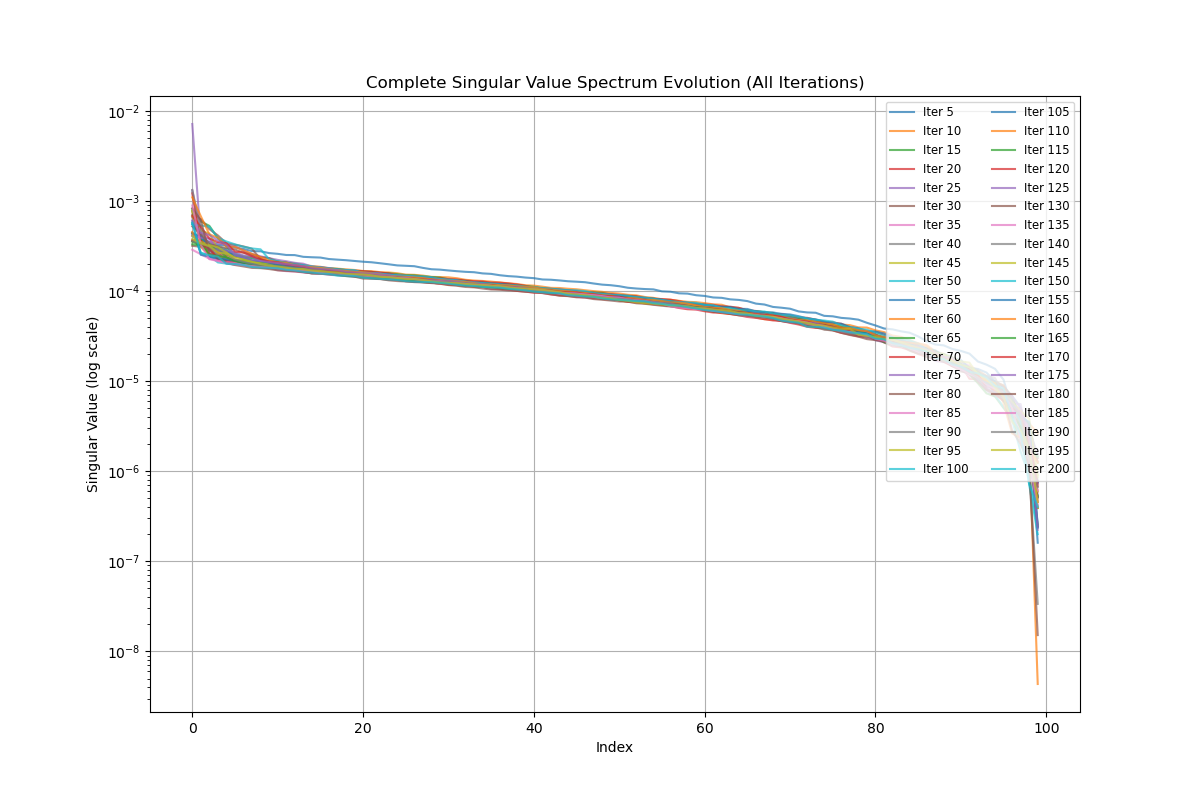
\includegraphics[width=0.8\linewidth]{../figs/mlp24/svd_evolution_all.png}}
        \caption{Singular values of random 100 parameters via 200 iterations}
        \label{fig:svd_all}
    \end{figure}
    \begin{figure}[h!]
        \center{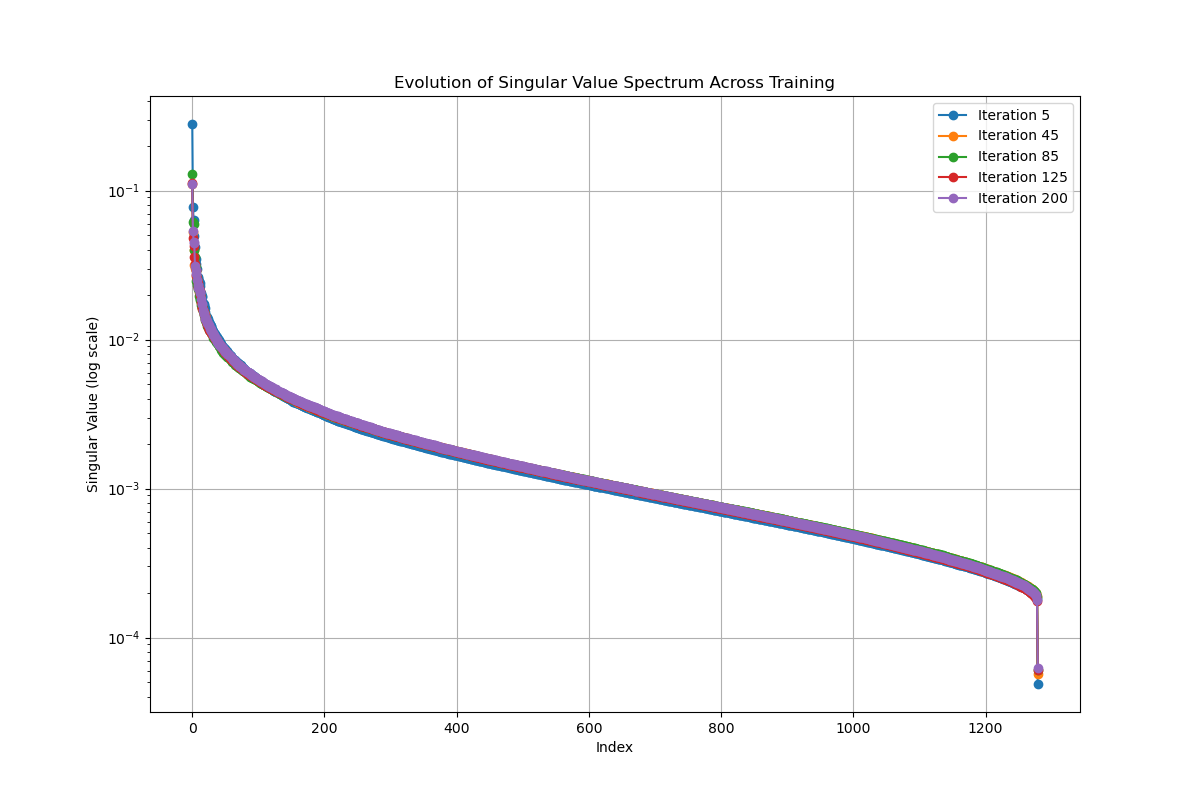
\includegraphics[width=0.8\linewidth]{../figs/mlp24/svd_evolution.png}}
        \caption{Singular values of random 100 parameters for 5-th,45-th, 65-th,175-th and 200-th iteration}
        \label{fig:svd}
    \end{figure} 
    
    \item NanoGPT is tested on Muon and Adam (add fig). The results are strange, because the methods do not converge at the expected rate (Muon is slower). Besides, Neon (rank-1 version) does not converge (see Figures ~\ref{fig:train_loss} \ref{fig:val_loss})
    \begin{figure}[h!]
        \center{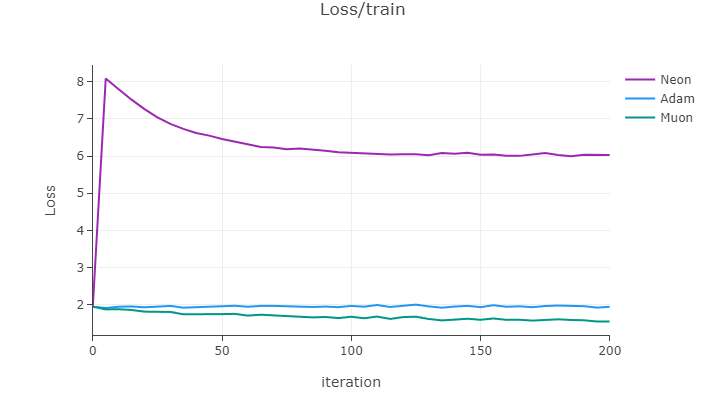
\includegraphics[width=0.8\linewidth]{../figs/mlp24/loss_train.png}}
        \caption{Train loss}
        \label{fig:train_loss}
    \end{figure}
    \begin{figure}[h!]
        \center{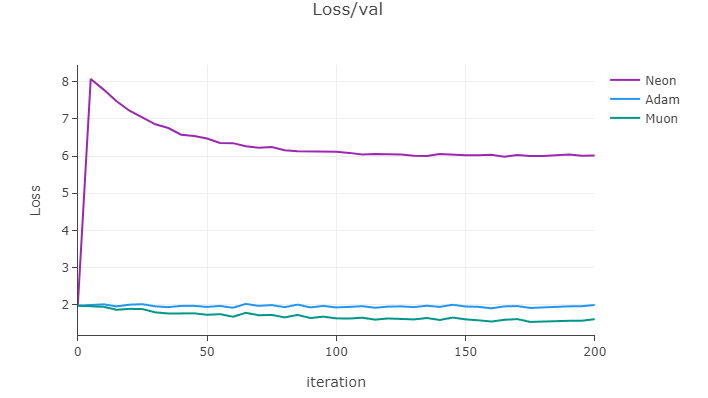
\includegraphics[width=0.8\linewidth]{../figs/mlp24/loss_val.png}}
        \caption{Validation loss}
        \label{fig:val_loss}
    \end{figure} 


    The pictures show the best results achieved so far. The experiments were conducted with two 4090 24GB GPUs for nanotgpt-large on the tiny stories dataset
    
    \item Neon (rank-1 version), Muon, AdamW and SGD are compared on MLP and CNN (see Figures~\ref{fig:mlp_epochs}, \ref{fig:cnn_epochs}, \ref{fig:mlp_time}, and~\ref{fig:cnn_time}). All methods work correctly, but again there is the problem with which one is the fastest (for now, it's SGD).
    \begin{figure}[h!]
        \center{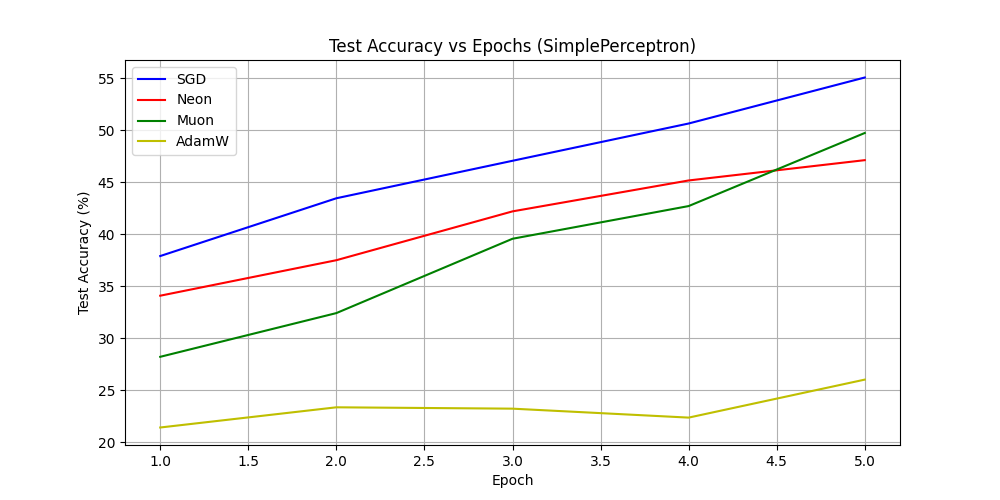
\includegraphics[width=0.8\linewidth]{../figs/mlp24/accuracy_vs_epochs_simple.png}}
        \caption{MLP: self.linear1 = nn.Linear(32*32*3, 512), self.linear2 = nn.Linear(512, 10), self.activ = nn.GELU()}
        \label{fig:mlp_epochs}
    \end{figure}
    \begin{figure}[h!]
        \center{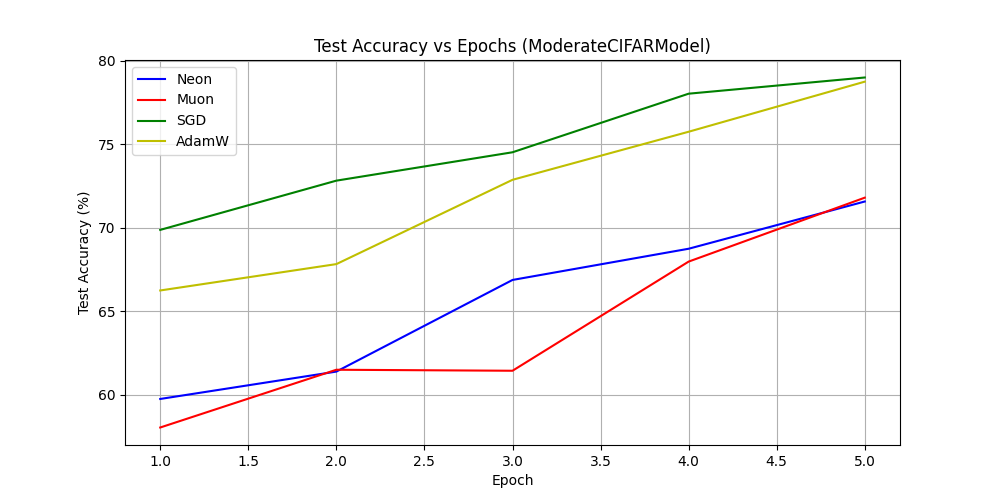
\includegraphics[width=0.8\linewidth]{../figs/mlp24/accuracy_vs_epochs_moderate.png}}
        \caption{CNN: 2 convolutional blocks, 2 fully connected layers, activation + dropout}
        \label{fig:cnn_epochs}
    \end{figure}
    \begin{figure}[h!]
        \center{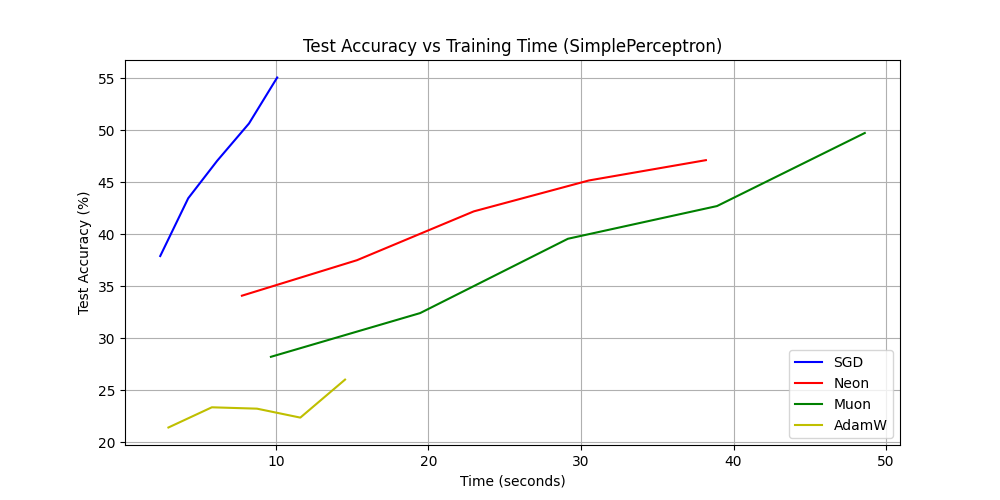
\includegraphics[width=0.8\linewidth]{../figs/mlp24/accuracy_vs_time_simple.png}}
        \caption{MLP: wallclock time measurements}
        \label{fig:mlp_time}
    \end{figure}
    \begin{figure}[h!]
        \center{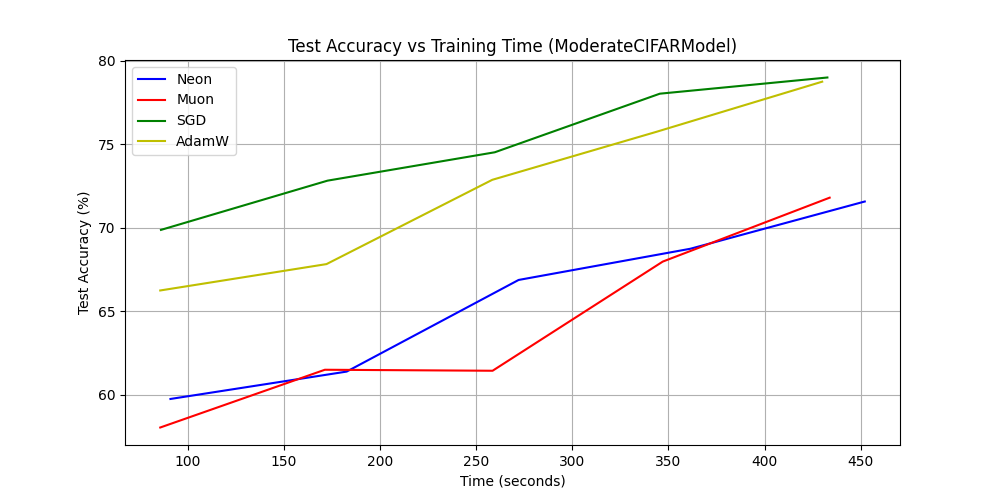
\includegraphics[width=0.8\linewidth]{../figs/mlp24/accuracy_vs_time_moderate.png}}
        \caption{CNN: wallclock time measurements}
        \label{fig:cnn_time}
    \end{figure}
\end{enumerate}\\



\bibliographystyle{unsrt}
\bibliography{muon.bib}

\end{document}
